	\subsection{Introducción}
	La presente obra es un informe descriptivo del banco para medición de figura de ruido presente en la Fundación CENDIT.
	Este sistema esta constituido casi en su totalidad por equipos de Agilent Technologies, es descrito en una nota de	aplicación como un sistema destinado a pruebas con fuentes de ruido, entre ellas, su calibración.
	
	\subsection{Objetivo}
	Por medio de una descripción general del sistema y una descripción de carácter técnico de cada uno de sus componentes, se pretende lograr un visión general acerca del uso y situación actual del banco de medición de figura de ruido dentro del CENDIT.
	
	\subsection{Descripción general del sistema}
	En un resumen técnico de la empresa Agilent Technologies \cite{AGI01} se propone los equipos mostrados en la \ref{Fig:BancoPruebasFuenteRuido} como un sistema para realizar pruebas con fuentes de ruido, entre ellas su calibración, para aplicaciones de radio frecuencia
	(RF) y microondas (UW). De acuerdo a esta nota técnica, el sistema planteado estaría compuesto por tres equipos
	fundamentales de Agilent Technologies, asociados con equipos periféricos de interconexión y apoyo.
	
	\begin{itemize}
		\item Un analizador de figura de ruido, modelo N8975A.
		\item Un controlador de interruptores y atenuadores, modelo 11713A.
		\item Un banco de atenuadores y aisladores, modelo N2002A.
	\end{itemize}	

	\begin{figure}[h!]			
		\centering
		\includegraphics[width=8cm]{Imagenes/EquiposSistemaMedicionRuido.pdf}
		\caption{Banco para pruebas con fuentes de ruido, propuesto por Agilent Technologies}
		\label{Fig:BancoPruebasFuenteRuido}
	\end{figure}

	El sistema incluye además fuentes de ruido, cables de interconexión y adaptadores coaxiales, algunos de los cuales se aprecian en la figura \ref{Fig:BancoPruebasFuenteRuido}.
	
	Si la caracterización de fuentes de ruido bien puede realizarse con un analizador de figura de ruido, como el equipo N8975A de la figura \ref{Fig:BancoPruebasFuenteRuido}, la empresa Agilent sugiere emplear dos dispositivos adicionales, si se desea disponer de la instrumentación adecuada para calibración de fuentes de ruido con elevada exactitud y trazabilidad. 
	
	De acuerdo a Agilent, un factor que degrada la exactitud y aumenta la incertidumbre en las mediciones de parámetros de ruido, es la interacción que existe a la salida de la NS y la entrada de señal del NFA, debida a ligeros desacoples de impedancia. Se emplearían entonces un banco de aisladores y atenuadores, el dispositivo Agilent N2002, interpuesto en el camino de señal, entre la salida de la fuente de ruido y la entrada del NFA, con el objeto de disminuir la interacción entre la NS y NFA para asi lograr medidas de elevada exactitud y baja incertidumbre.
	
	Como dispositivo N2002 no presenta interfaz de usuario ni posee “inteligencia” interna que permita comandarlo, requiere de un dispositivo controlador externo, un equipo de la serie 11713 de Agilent. Por medio de la interfaz que dispone el 11713, el usuario realiza la selección de la atenuación requerida en el banco de atenuadores N2002A.
	
	Las mediciones de potencia de ruido en dispositivos RF y UW exige fuentes de ruido calibradas si se desea una elevada precisión y exactitud, el error en dichas mediciones esta fuertemente ligado a la incertidumbre de la fuente de ruido	empleada. Por ello es de vital importancia su calibración, entendida esta como la verificación que se realiza en los	parámetros de la fuente de ruido para asegurar que la misma se encuentra dentro de los valores nominales establecidos	por la calibración de fabricante. 
	
	Por medio del sistema propuesto por Agilent, se puede calibrar las fuentes de ruido “en casa”, sin depender de laboratorios de calibración externos.
	
	Uno de los pasos en el proceso de calibración de fuentes de ruido es la medición de la razón de ruido en exceso \emph{ENR} (\emph{Excess Noise Ratio}) de la fuente en cuestión. Si bien este paso de la calibración puede realizarse empleando únicamente un analizador de figura de ruido, la motivación de Agilent al presentar este sistema es que utilizando los dispositivos N2002A y 11713A en conjunto con el analizador de figura de ruido se pueden lograr mediciones de ruido con mayor exactitud. 
	
	Sin embargo, el sistema no esta limitado únicamente a realizar calibración de fuentes de ruido, permite además realizar	cualquier tipo de medición relacionada con ruido en RF y UW, como mediciones de potencia de ruido, figura de ruido, temperatura equivalente de ruido, razón de ruido en exceso y mediciones de ganancia de potencia.
	
	\section{Estado del banco para pruebas con fuente de ruido en el CENDIT}
	El banco para pruebas con fuentes de ruido dentro del CENDIT se encuentra incompleto, ya falta uno de los tres equipos integrantes de este sistema. El CENDIT dispone del analizador de figura de ruido N8975A y del banco de atenuadores y aisladores N2002, pero hasta la fecha no ha logrado la adquisición del 11713A, el modelo antiguo producido por Agilent para la unidad controlador de interruptores y atenuadores, o de los modelos más recientes para este equipo, el 11713B o 11713C, actualmente fabricados por Keysight Technologies.
	
	Dificultades en la procura de equipos desde el exterior, han impedido al CENDIT adquirir un cualquier equipo de la serie 11713. El CENDIT se ha propuesto diseñar y desarrollar una replica de este equipo, funcionalmente equivalente a los equipos de la serie 11713, en sus instalaciones. Ha delegado esta tarea como un tema de tesis en el pasante Br. Jose Arias, autor del presente informe.
	
	A continuación se da un inventario de equipos que cuenta el CENDIT para implementar el banco para pruebas con fuentes de ruido.
	
	\subsection{Inventario del sistema equipos}
	
	\subsubsection{Equipos}	
		~		
		
		\begin{table}[h!]
			\centering
			
			\begin{tabular}{|c|c|c|c|}
				\hline
				 Modelo & 	Descripción &  Fabricante & Cantidad \\
				\hline
				 N8975A &	Analizador de figura de ruido &  Agilent &  1  \\
				\hline
				 N2002 	& 	Equipo para pruebas con fuente de ruido & Agilent &  1 \\ 
				\hline
				 E5810 	& 	Puente red LAN a bus GPIB / RS232 &  Agilent &  1 \\
				\hline
				 82357B &  Adaptador bus USB a bus GPIB  & Agilent &  2 \\
				\hline
				
			\end{tabular}
		\end{table}

	\subsubsection{Fuentes de ruido}	
	 	~	 	
	 	
		\begin{table}[h!]
			\centering
						
			\tablefirsthead{}
			\tablehead{}
			\tabletail{}
			\tablelasttail{}
			\begin{tabular}{|c|c|c|c|}
				\hline 
				Modelo 	& 	Descripción & Fabricante & Cantidad \\ 
				\hline
				 N4000A & 	Fuente de ruido SNS ENR nominal de 6 dB & Agilent & 1 \\ 
				\hline
				 N4001A & 	Fuente de ruido SNS ENR nominal de 15 dB & Agilent & 1 \\ 
				\hline
				 N4002A &	Fuente de ruido SNS ENR nominal de 14 dB & Agilent & 1 \\
				\hline
			\end{tabular}
		\end{table}
	
	\subsubsection{Cables}	
		~		
		
		\begin{table}[h!]
			\centering
						
			\tablefirsthead{}
			\tablehead{}
			\tabletail{}
			\tablelasttail{}
			\begin{tabular}{|c|c|c|c|}
				\hline
				 Modelo & Descripción & Fabricante & Cantidad \\
				\hline
				 11730A & Cable para fuente de ruido SNS & Agilent & 3 \\
				\hline
				 10833A & Cable conexión bus GPIB, 1 metro & Agilent & 2 \\
				\hline
				 10833B & Cable conexión bus GPIB, 2 metros & Agilent & 2 \\
				\hline
				 11500E & Cable coaxial de 3.5 mm – (m-m) & 	~	& 1 \\
				\hline
			\end{tabular}
		\end{table}
	
	\subsubsection{Adaptadores coaxiales}	
		~		
		
		\begin{table}[h!]
			\centering
						
			\tablefirsthead{}
			\tablehead{}
			\tabletail{}
			\tablelasttail{}
			\begin{tabular}{|c|c|c|c|}
				\hline
				 Modelo 	& Descripción & Fabricante & Cantidad \\
				\hline
				 1250-1744 	& Adaptador coaxial Tipo N (m) a 3.5 mm (f) & Agilent & 1 \\
				\hline
				 1250-1745 	& Adaptador coaxial Tipo N (f) a 3.5 mm (f) & Agilent & 1 \\
				\hline
				 1250-1750 	& Adaptador coaxial Tipo N (f) a 3.5 mm (m) & Agilent & 1 \\
				\hline
				 83059A 	& Adaptador coaxial de 3.5 mm (m) a (m) & Agilent &	 1 \\
				\hline
				 83059B 	& Adaptador coaxial de 3.5 mm (f) a (f) & Agilent & 1 \\
				\hline
			\end{tabular}
		\end{table}
	
	\subsubsection{Accesorios}	
		~		
		
		\begin{table}[h!]
			\centering			
			
			\tablefirsthead{}
			\tablehead{}
			\tabletail{}
			\tablelasttail{}
			\begin{tabular}{|c|c|c|c|}
				\hline
				 Modelo	 	& Descripción & Fabricante & Cantidad \\
				\hline
				 E5810-100 	& Kit para montaje en rack del E5810 & Agilent & 1 \\
				\hline
			\end{tabular}
		\end{table}
	
	\clearpage
	
	\section{Sistema de medición de figura de ruido}
	
	En la figura \ref{Fig:EsquemaSistemaMedicion} se muestra un diagrama conceptual para el sistema de medición de figura de ruido, objetivo de implementación dentro del CENDIT, cumplirá dos tareas principales serán la medición de figura de ruido en dispositivos de RF y {\textmu}W y la calibración de fuentes de ruido.
	
	\begin{figure}[h!]
		\centering
		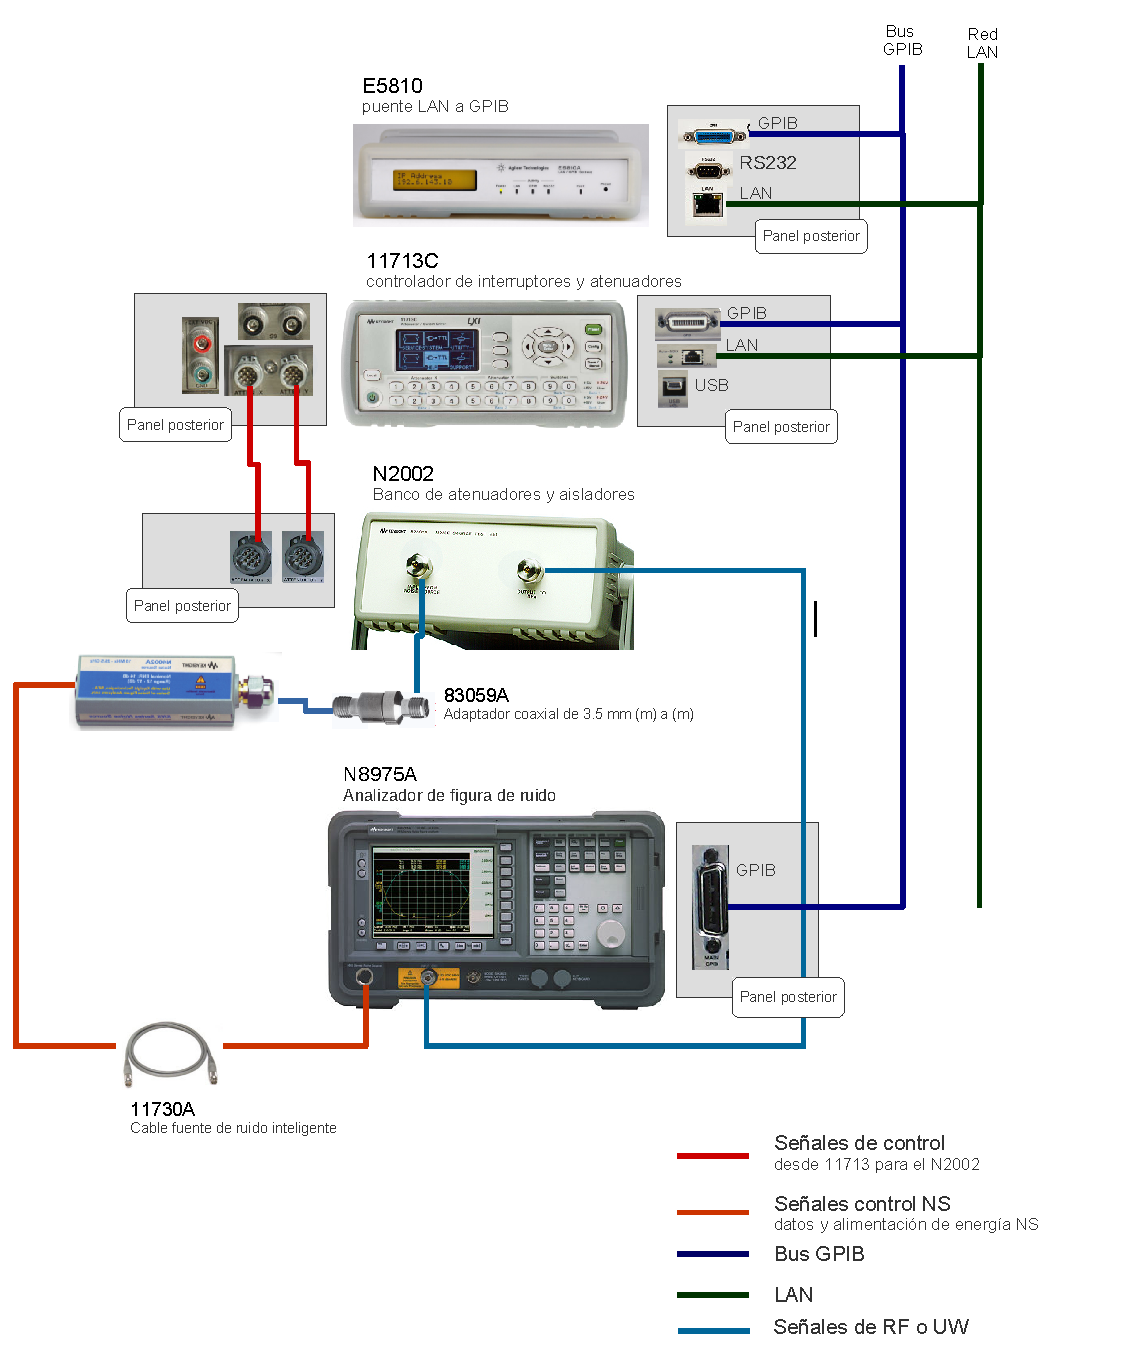
\includegraphics[height=17cm]{Imagenes/SistemaMedicionFiguraRuido.pdf}
		\caption{Sistema para medición de figura de ruido}
		\label{Fig:EsquemaSistemaMedicion}
	\end{figure}
	
	Se aprecia en la figura \ref{Fig:EsquemaSistemaMedicion} que el sistema es el resultado de la integración de equipo de hardware, interconectado por un conjunto de vías de señal y buses para transmisión de datos más una capa de aplicaciones de software. El sistema permitirá la medición de parámetros de relativos al ruido como lo son la potencia de ruido, temperatura efectiva y figura de ruido, su presentación gráfica, almacenamiento y distribución en red.
	
	Es un sistema la resultante de la integración de equipo hardware y aplicaciones de software, la tarea esencial es la	medición de la figura de ruido en dispositivos.  Permite la medición de parámetros de ruido, su presentación, análisis almacenamiento y distribución en red. No solo de forma local sino de manera remota, empleando sus capacidades de	conexión a buses.
	
	El núcleo del sistema lo representa el analizador de figura de ruido (NFA) N8975 y las fuentes de ruido inteligentes (Smart Noise Source, SNS) de la serie N4000A, ambos productos de Agilent. Las capacidades del NFA definen la funcionalidad de todo sistema: es el encargado de la medición, presentación, almacenamiento y distribución de datos relativos a la figura de ruido. 
	
	Las fuentes de ruido inteligentes constituyen una fuente de señal de referencia de \ RF y de UW. Estas generan una señal de ruido blanco, con niveles de potencia conocidos. 
	
	Empleando el NFA en conjunto con una SNS es posible medir la figura de ruido en un dispositivo o verificar la calibración de una fuente de ruido. Agilent propone anteponer a la entrada del NFA un banco de atenuadores y aisladores, el dispositivo N2002A en la figura \ref{Fig:EsquemaSistemaMedicion}, como un mecanismo para aumentar la exactitud y reducir la incertidumbre en las mediciones.
	
	El N2002A es un dispositivo que carece interfaz de usuario, es necesario emplear un equipo de la serie 11713 \textemdash actualmente producidos por Keysight Technologies \textemdash, conocido como unidad controladora de interruptores y atenuadores (\ref{Fig:EsquemaSistemaMedicion}). 
	
	El equipo 11713B (\ref{Fig:EsquemaSistemaMedicion}) presenta una interfaz sobre la cual el usuario selecciona el rango de frecuencias sobre el	cual el N2002A debe dejar pasar en el camino de señal. El 11713B traduce las pulsaciones del usuario en los botones frontales a señales de control apropiadas que permiten establecer las frecuencias de paso en el N2002A. Estas señales	se transmite por medio de un cables especiales conectados en los puertos ubicados en los paneles traseros de ambos equipos.
	


